\documentclass[11pt]{article}
\setlength{\topmargin}{-0.25in}
\setlength{\textheight}{8.75in}
\setlength{\oddsidemargin}{.125in}
\setlength{\textwidth}{6.25in}
\linespread{1.4}
\usepackage{graphicx}
\usepackage{chemmacros}
\usepackage{amsmath}
\usepackage{float}
\usepackage{gensymb}
\usepackage{multirow}
\usepackage{color}
\usepackage{wrapfig}
\usepackage{tabularx}
\usepackage[font=small,labelfont=bf]{caption}
\author{N. Belliveau, G. Chure, J. Theriot, R. Phillips}

\begin{document}
\title{Supplemental Information}
\maketitle

\section{Summary of Proteome Datasets.}

Here we briefly summarize the datasets that were considered for the work of the main
text. The goal of this section is to give an overview of each dataset
considered, including the main experimental details, and to provide a more
detailed look at how well each compares.

Table \ref{table:datasets} provides an overview of the proteomic datasets that
we found in the literatrue. These are predominately mass spectrometry-based,
with the exception of the work from Li {\it et al.} (2014) which used ribosomal
profiling, and the fluorescence-based counting done in Taniguchi {\it et al.}
(2010). The general strategy taken in these works is to quantify fractional
abundance of each protein and then to convert these to absolute abundance by
multiplying these fractions by the bulk measusured total cellular protein
abundance. Note that the work of Peebo {\it et al.} (2014) did not perform any
measurement of cell count or volume, and thus were only able to report cellular
protein concentration.

Exceptions to this are found in Schmidt {\it et al.} and Taniguchi {\it et al.}.
A key distinction in the work of Schmidt {\it et al.} is that in addition to
determining relative abundance by mass spectrometry, they also selected 41
enzyme that cover over four orders of magnitude in cellular abundance to use in
absolute protein quantification. Specifically, synthetic peptides were generated
for each of these 41 enzymes and used to provide a calibration between measured
mass spectrometry intensities and absolute protein abundances (using stable
isotope dilution (SID) and selected reaction monitoring (SRM), though the
details of this are beyond the scope of this section). In the work of Taniguchi
{\it et al.},  the authored tagged each protein with a  yellow fluorescent
protein (YFP) and used fluoresence as readout of cellular expression.


% \begin{center}
\begin{tabularx}{.8\textwidth}{ || c | c | c | c | c | c | c || }
\hline
Author & Method & Strain & $N$ datasets & Reported Quantity & fractional coverage (by count) & fractional coverage (by mass) \\
\hline\hline
Taniguchi {\it et al.} (2010) & YFP-fusion, cell fluorescence  & & & fg/copies per cell & & \\
\hline
Valgepea {\it et al.} (2012) & Mass spectrometry  & & & fg/copies per cell & & \\
\hline
Peebo {\it et al.} (2014) & Mass spectrometry  & & & fg/copies per fL & & \\
\hline
Li {\it et al.} (2014) & Ribosomal profiling  & & & protein synthesis rate & & \\
\hline
Soufi {\it et al.} (2015) & Mass spectrometry  & & & fg/copies per cell & &\\
\hline
Schmidt {\it et al.} (2016) & Mass spectrometry  & & & fg/copies per cell & & \\
\hline
Caglar {\it et al.} (2017) & Mass spectrometry  & & & relative abundance & &\\
\hline
\end{tabularx}
% \label{table:datasets}
% \end{center}

Figure \ref{} shows the distribution in reported protein abundance for   a  subset
of  the data.

An important consideration is whether the reported abundance per cell are correlated. while
we expect some variability in expression of each protein due to growth rate, the reported
values are nonetheless expected to be correlated. Figure \ref{fig:dataset_correlations} compares each dataset to the copy numbers from Schmidt {\it et al.}, grown in M9 minimal media supplemented with glucose.

\begin{figure}[H]
		\centering
    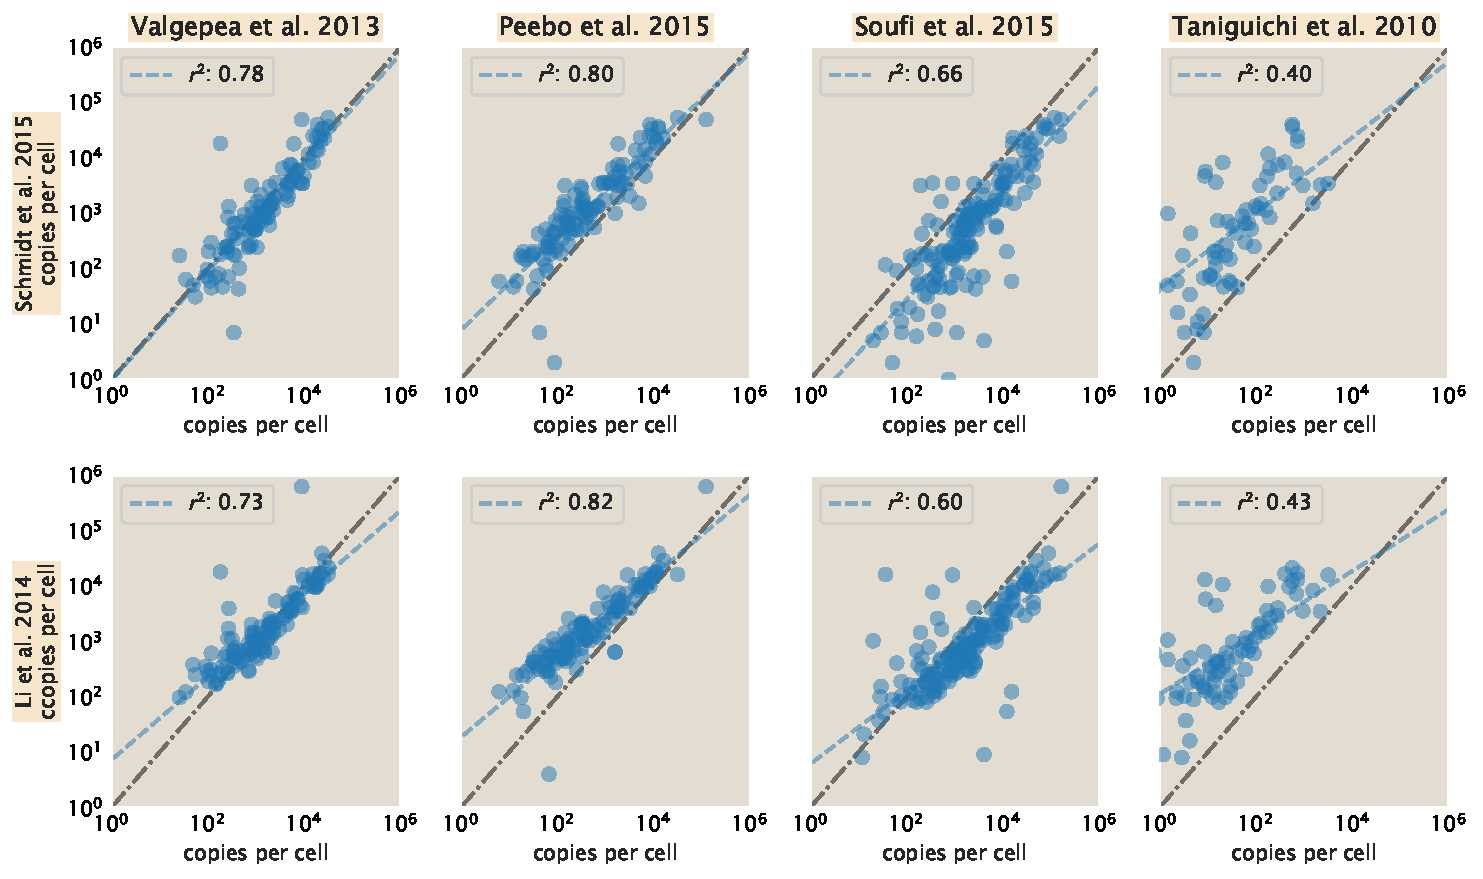
\includegraphics[width=1\textwidth]{../../figures/dataset_correlations.pdf}
  \caption{}
  \label{fig:dataset_correlations}
\end{figure}

\begin{figure}[H]
		\centering
    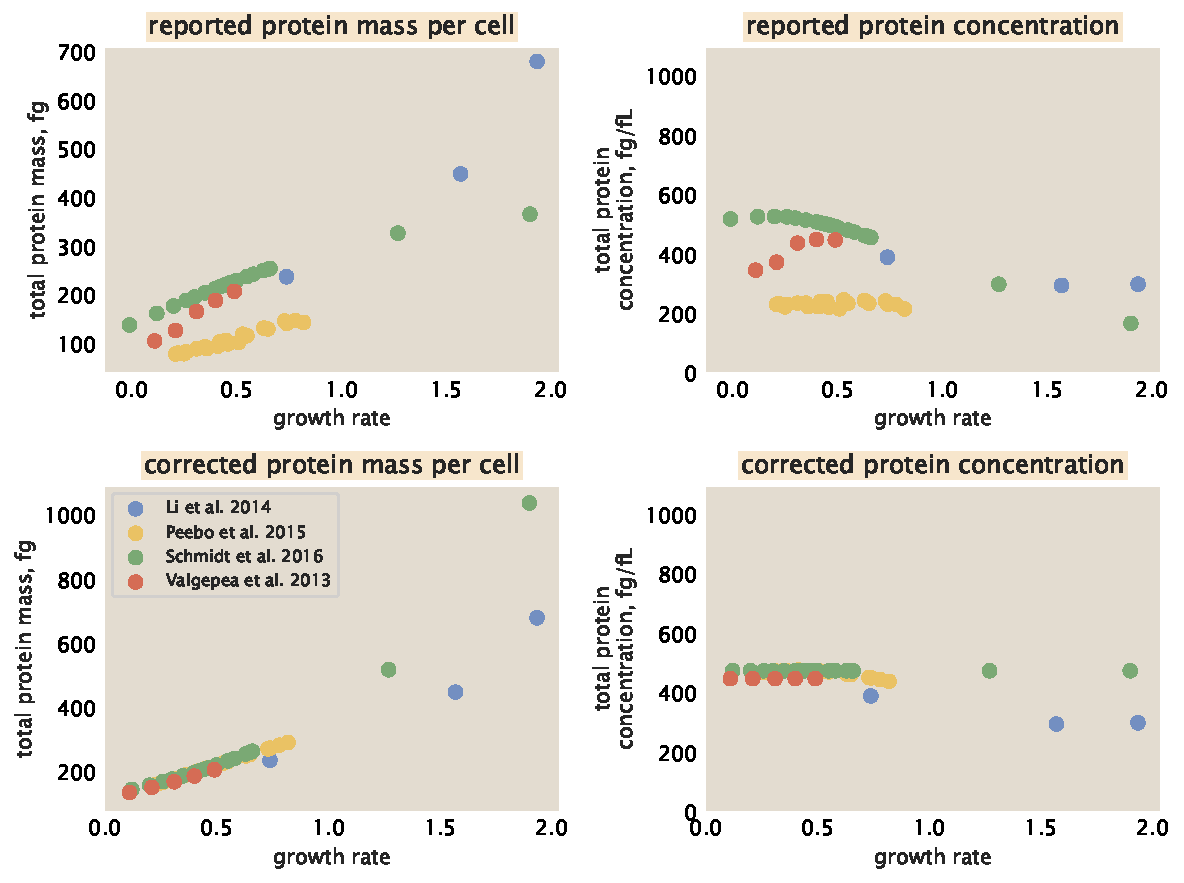
\includegraphics[width=1\textwidth]{../../figures/dataset_corrections.pdf}
  \caption{}
  \label{fig:dataset_correlations}
\end{figure}


\section{Adjustments to Copy Number Data.}

% NB: need to make summary figure with 2x2 panels; top row A) reported total protein per cells
% B) protein concentration. bottom row, C) new total protein mass per cell,
% C) new protein concentration.

% NB: It may be helpful to appeal to the 'classic growth laws' early on in this text
% as a rational to guide thinking with expections about total cell mass, cell volume w.r.t.
% growth rate.

The datasets encompass a range of bacterial growth conditions,  different {\it
e. coli} strains, and for those that report quantities on a cell basis,
different methods to normalize  by  cell count and volume. It was therefore
important to consider if certain discrepencies exist across the data and whether
these might be reasonably dealt with to make the compilated dataset internally
consistent. - give reference to what was done in example of yeast proteome data
corrections. However, given the work of [cite] and others, there are
well-documented expectations about how characteristics such as total protein
mass per cell and cell volume  should scale with growth rate. We were therefore
inclined to only renormalize data in a  way  that took into account such
expectations. Figure \ref{} shows the total protein  mass reported as a function
of growth rate for each experiment. Indeed, with the exception of the work of
Peebo et al., the total mass per cell is generally consistent as a fuction of
growth rate, and provide some confidence in such an approach.

In the remainder of this section we describe the rescaling that was done to each
dataset, with a particular focus on correcting for discrepencies in cellular
protein concentration, which may reflect differences in protein extraction
efficiency. It is important to note that with the exception of the work from
Peebo {\it et al.} (which is discussed more below), any rescaling is only
performed within the data of individual authors and not performed globally. We
felt this was important in order not to bias any individuals' work since we lack
any true standard of protein abundance.

% for differences in
% cellular protein concentration within each inidividual dataset. This  strategy
% was already applied in the work of Schmidt et al., in particularr due to
% concerns  over lower protein extraction efficiency in growth conditions like
% stationary phase.  However, another complicating factor that became apparent is
% a descrpency in expected versus reported cell volume that required additional
% care and is further described below. Lastly, the  data from Peebo {\it et al.}
% required additional care due to a lack quantities on a cell basis, and we
% consider this work seperately.


\subsection{Corrections to Enforce a Consistent Cellular Protein Concentration}

% NB: It may be useful to note that none of this should have any effect on the relative
% abundances found in each dataset.

One parameter that we do not expect to change substantially across growth
conditions is cellular protein concentration. As a general rule of thumb, we
expect an {\it e. coli} cell to have about 30\% dry mass, with about 55\% of
this expected from protein. With a density of about 1.1 g/ml, we find that the
protein concentration in a cell should be approximately 180 fg/fL.  The cellular
density and dry mass are essentially fixed, with the fraction of cellular
protein varying from [X-Y; refs??]. Hence,  this parameter provides a useful
reference point that datasets should agree on.  Indeed, out of concern over
differences in protein extraction efficiency in growth phases like stationary
phase, Schmidt {\it et al.} applied a correction to their measured protein
abundances to ensure cellular protein concentrations were internally consistent.


From the work of Schmidt {\it et al.} they reported an ability to consistently get high
protein yield from cells grown in M9 minimal media supplemented with glucose. In order
to account any protein loss during extraction, they use their measured protein concentration
from this sample as a reference for which total protein concentration in all other growth
conditions should match. This is shown in Figure \ref{}A. One challenge in
performing this calculation is that cell volume must be known; the authors use
volumes that were  measured by flow cytometry in previous work [cite]. These
volumes are shown in Figure \ref{}B. While it is difficult to assess the
accuracy of these numbers, we find them to be quite inconsistent with the
expected scaling that is reported by Taheri-Araghi {\it et al.} (2015),
carefully
measured as a function of growth rate [and other work?].

In addition,  since cell volume was not determined in all studies, and to be
consistent throughout, we instead use the predicted cell volumes from
Taheri-Araghi {\it et al.}. Dealing with each dataset seperately, we apply
correction  factors to correct for discrepencies in protein concentration across
the different growth conditions considered [NB: I wonder if in these other
datasets, the more appropriate thing to do is match to the average measured
protein concentration]. Specifically, the scaling factor $\phi$ is given by,

\begin{equation}
\phi  =  \frac{P_i}{V_i} \cdot [P]_r
\end{equation}

where $P_i$ is the total protein mass in conditino $i$, $V_i$ is the estimated cell volume, and $[P]_r$ is
the reference protein concentration (i.e. growth in  glucose for the Schmidt data).


\subsection{Peebo {\it et al.}: Conversion from copies/ fL to copies per cell}

In the work of Peebo {\it et al.}, the authors only report protein concentration.
In  order to determine protein per cell, we multiple these concentrations by
expected cell volumes  using the predictions from  Taheri-Araghi {\it et al.} This is
shown in Figure \ref{}A, where we see that reported mass is substantially lower than
the other work considered here; as well as work from others [Sinauer, 1990].

Indeed, both Schmidt {\it et al.} and Li {\it et al.} reported a total protein mass of about
250 fg per cell at a growth rate of about $\lambda \approx 0.5 hr^{-1}$ ( M9
minimal media with glucose and MOPS minimal media, respectively). Given this
descrepency, in addition to requiring that cellular protein concentration be
internally consistent across the growth conditions they reported on, we also
required that total cellular mass be consistent with the work Schmidt {\it et al.} and
Li {\it et al.} This amounted to performing a linear regression between total protein
mass and growth rate, and using this to scale the Peebo {\it et al.} dataset according
to this trend.


 % cell biology by the numebrs: Overall macromolecular composition of an average
 % E. coli cell in aerobic balanced growth at 37°C in glucose minimal medium,
 % with doubling time of 40 minutes and 1 pg cell wet weight (≈0.9 μm^3 cell
 % volume). Adapted with modifications from F. C. Neidhardt et al., “Physiology
 % of the bacterial cell”, Sinauer, 1990 (BNID 104954). Modifications included
 % increasing cell dry weight from 284 fg to 300 fg and total cell mass from 950
 % to 1000 fg as

%



\end{document}
